\chapter{Εισαγωγή}

%Το \en{Lorem Ipsum} είναι απλά ένα κείμενο χωρίς νόημα για τους επαγγελματίες της τυπογραφίας και στοιχειοθεσίας \cite{LoremIpsumAll}. Το \en{Lorem Ipsum} είναι το επαγγελματικό πρότυπο όσον αφορά το κείμενο χωρίς νόημα, από τον 15ο αιώνα, όταν ένας ανώνυμος τυπογράφος πήρε ένα δοκίμιο και ανακάτεψε τις λέξεις για να δημιουργήσει ένα δείγμα βιβλίου. Όχι μόνο επιβίωσε πέντε αιώνες, αλλά κυριάρχησε στην ηλεκτρονική στοιχειοθεσία, παραμένοντας με κάθε τρόπο αναλλοίωτο. Έγινε δημοφιλές τη δεκαετία του '60 με την έκδοση των δειγμάτων της \en{Letraset} όπου περιελάμβαναν αποσπάσματα του \en{Lorem Ipsum}, και πιο πρόσφατα με το λογισμικό ηλεκτρονικής σελιδοποίησης όπως το \en{Aldus PageMaker} που περιείχαν εκδοχές του \en{Lorem Ipsum}.
Φαίνεται ότι ο χρόνος που σπαταλάνε οι μηχανικοί δικτύωσης όταν εισέρχονται σε εξοπλισμό δικτύωσης για να εισάγουν χειροκίνητα εντολές οπως για τη διαμόρφωση των συσκευών ή να εισέρχονται σε διακομιστές για τη χειροκίνητη
ρύθμιση μία προς μία μια λίστα συσκευών/δικτύων(\en{access lists}) είναι πολύ μεγάλος, συνεπώς η εποχή που όλα αυτά γινόντουσταν χειροκίνητα φτάνει στο τέλος της. Όλο και περισσότεροι/περισσότερες εταιρείες προωθούν την αυτοματοποίηση καθώς βλέπουν ότι κάθε
ώρα που επενδύεται στην αυτοματοποίηση μεταφράζεται σε πολλές ώρες εργασίας που εξοικονομούνται. 

Η αυτοματοποίηση αυτών των εργασιών με κάποια καλοφτιαγμένη λογική προγραμματισμού επιτρέπει
τη διαμόρφωση εκατοντάδων συσκευών μέσα σε λίγα λεπτά, απομακρύνει τη δυνατότητα
των λανθασμένων ρυθμίσεων που προέρχονται από ανθρώπινο λάθος, επιτρέπει την καταγραφή των αλλαγών διαμόρφωσης και έχει το πλεονέκτημα ότι καθιστά τη διαμόρφωση
τεχνικές λεπτομέρειες διαφανείς στον χρήστη που πρόκειται να ξεκινήσει τη διαδικασία αυτοματοποίησης. Για παράδειγμα, μια εταιρεία θα μπορούσε να αναθέσει υπεργολαβικά σε μια ομάδα λειτουργίας
που δεν έχει τεχνικές γνώσεις δικτύωσης και απλά παρέχοντάς τους μια
συγκεκριμένο σύνολο εισόδων θα μπορούσαν να διαμορφώσουν για Χ σημεία πρόσβασης σε Υ δίκτυα
ένα συγκεκριμένο SSID με τις επιθυμητές παραμέτρους. Οι δεδομένες είσοδοι θα μπορούσαν
να εισαχθούν από αυτούς σε μια εφαρμογή ιστού και ο υποκείμενος προγραμματισμός
κώδικας θα έκανε τα υπόλοιπα. Τελικά αυτό μεταφράζεται σε ένα πολύ γρήγορο και αξιόπιστο πλάνο κατά το οποίο η παραμετροποίηση και η
διαμόρφωση ενός δικτύου δεν θα χρειάζεται να γίνει από τους μηχανικούς δικτύωσης χειροκίνητα.

Μπορούν να επενδύσουν συνεπώς αυτόν τον επιπλέον χρόνο σε άλλες εργασίες όπως ο σχεδιασμός και έτσι οι πιο χρονοβόρες διαδικασίες να αυτοματοποιηθούν. Αλλά η αυτοματοποίηση δεν είναι μόνο
κάνει θαύματα όσον αφορά τη διαμόρφωση, είναι επίσης εξαιρετική για την παρακολούθηση της κατάστασης των δικτύων/συσκευών/θυρών, την απόκτηση πληροφοριών για την υγεία των ασύρματων δικτύων και κάθε
άλλες πληροφορίες που μπορούν να λάβουν από της δυκτυακές συσκευές.

Είναι σημαντικό να ληφθεί υπόψη ότι οι επαναλαμβανόμενες καθημερινές/εβδομαδιαίες εργασίες
που απαιτούν τη συλλογή πληροφοριών είναι εξαιρετικοί υποψήφιοι για αυτοματοποίηση.
Με μια αυτοματοποίηση που αναζητά τα απαιτούμενα δεδομένα και κάνει κάποια επεξεργασία οι απαιτούμενες πληροφορίες μπορούν να ληφθούν γρήγορα και να παρουσιαστούν στους
μηχανικό και τον/την απαλλάσσει από το να συνδέεται χειροκίνητα σε πολλές συσκευές, να ελέγχει
ορισμένων γραμμών διαμόρφωσης, κ.λπ.

Παράλληλα η επανάσταση που έφερε η εισαγώγή της λογικής των \en{microservices} στον κλαδο της Πληροφορικής μπορεί να καθιστήσει την εφαρμογή αυτή ακόμα πιο αξιόπιστη
γιατί μπορεί να συμβάλει στο σχεδίασμό ενός συστήματος λογισμικού με μεγαλύτερη αξιοπιστία καθώς και να προσφέρει όλες εκείνες της θετικές προεκτάσεις χρήσης αυτών.
Θα γίνει λοιπόν μια προσπάθεια εισαγώγής τεχνολογιών διαχείρισης και ανάπτυξης \en{microservices} όπως \en{kubernetes} και \en{containers}. Τα πλεονεκτήματα της χρήσης της αρχιτεκτονική \en{Microservices} είναι ότι προσφέρουν μεγαλύτερη ευελιξία 
μέσω της ανεξαρτησίας των υπηρεσιών, επιτρέποντας στους οργανισμούς να γίνουν πιο ευέλικτοι όσον αφορά τον τρόπο με τον οποίο προσφέρουν νέες επιχειρηματικές δυνατότητες ή ανταποκρίνονται στις μεταβαλλόμενες συνθήκες της αγοράς. Αναλυτική παρουσίαση αυτών θα γίνει σε επόμενο κεφάλαιο. 


\section{Απαιτήσεις και προδιαγραφές}
\begin{itemize}
    \item \en{GNS3 VM} ,\en{Cisco} \en{Images} και \en{GNS3} περιβάλλον
    \item \en{Vs Code development environment}
    \item \en{Virtual box} ή οποιονδήποτε \en{type B hypervisor}
\end{itemize}


%\begin{equation}
%	y = \alpha x + \beta
%\end{equation}

%Αντίθετα με αυτό που θεωρεί η πλειοψηφία, το \en{Lorem Ipsum} δεν είναι απλά ένα τυχαίο κείμενο. Οι ρίζες του βρίσκονται σε ένα κείμενο Λατινικής λογοτεχνίας του 45 π.Χ., φτάνοντας την ηλικία του πάνω από 2000 έτη.


%\begin{figure}[htb]
%	\centering
%	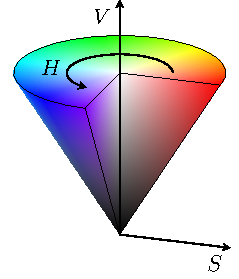
\includegraphics{tikz/hsv_cone/hsv_cone.pdf}
%	\caption{Ο χρωματικός χώρος \en{HSV}.}
%\end{figure}
